

\subsection{Ondelettes}
\subsubsection{Une brève introduction aux ondelettes}


Les ondelettes proviennent du monde du traîtement du signal. Elles répondent à un problème de représentation des données à la fois dans le domaine temporel et dans le domaine fréquentiel. En effet, la transformée de Fourier nous donne accès aux fréquences présentes dans un signal mais ne nous permet pas de localiser à quel moment sont intervenues les fréquences spécifiques. Le théorème d'indétermination de Heisenberg stipule que l'on ne peut avoir une résolution parfaite à la fois dans le domaine fréquentiel et le domaine temporel, il y a un compromis qui doit être fait. La question devient alors :

\question{
	\smallskip\centering
	Comment représenter une fonction dans le domaine temporel et dans le domaine fréquentiel de façon optimale ? En d'autres termes, quelle résolution temporelle et quelle résolution fréquentielle choisir ?
}

Une première approche proposée en 1946 par Denis Gabor est la transformée de Fourier à court terme (STFT). Celle-ci consiste à regarder la transformée de Fourier d'une fonction sur une fenêtre de taille fixe et à faire glisser cette fenêtre sur la fonction. On obtient ainsi la représentation fréquentielle de la fonction sur un intervalle de temps centré en un point que l'on peut faire varier.

\bigskip

\begin{minipage}{0.32 \textwidth}
	\begin{figure}[H]
		\centering
		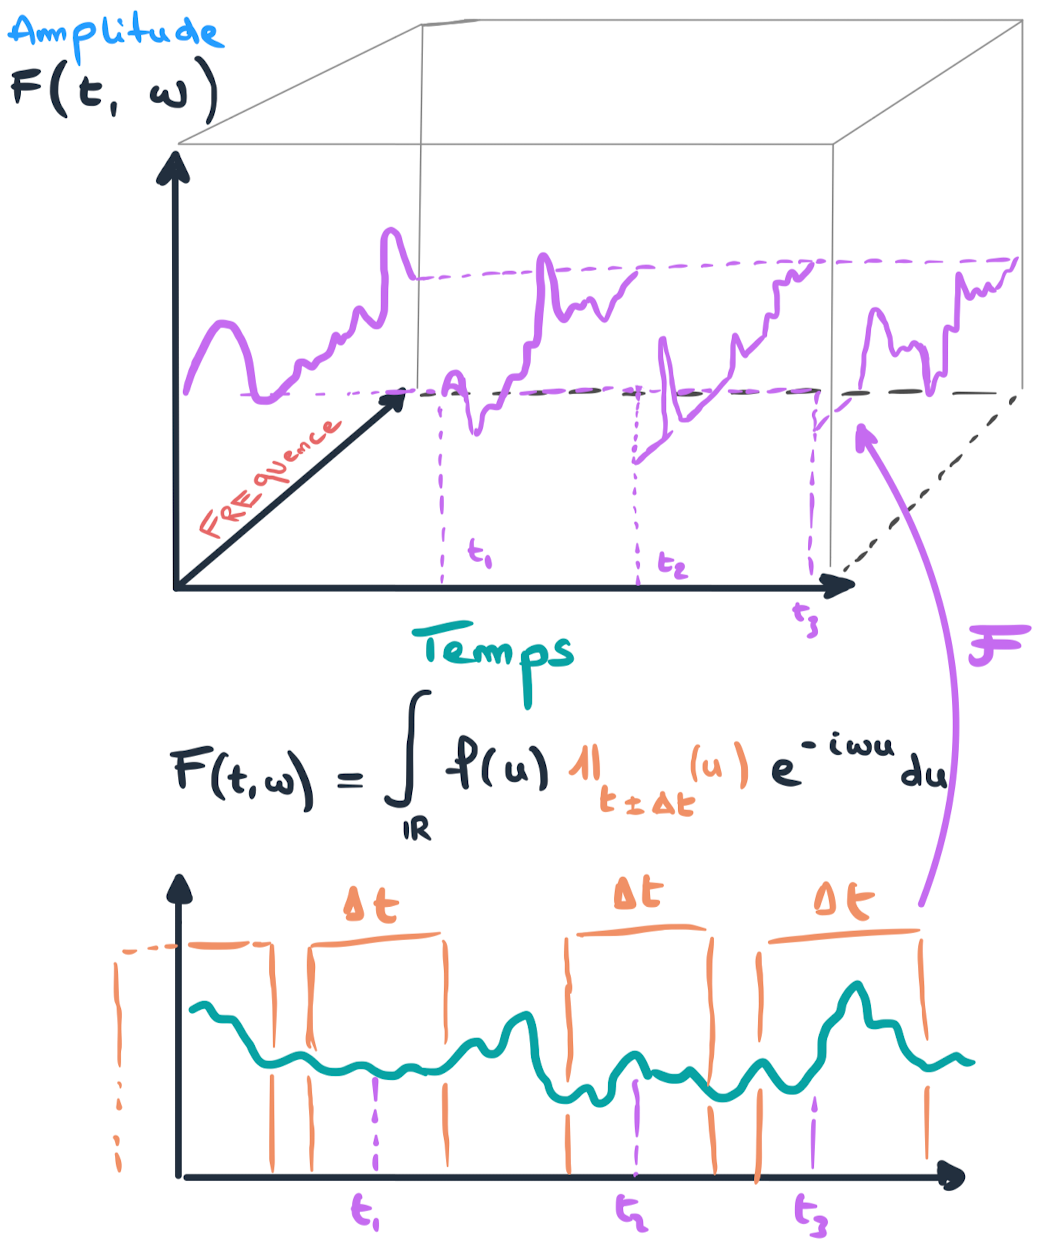
\includegraphics[width=\textwidth]{images/sketches/STFT.png}
		\caption{Transformée de Fourier à court terme d'une fonction}
		\label{fig:STFT}
	\end{figure}
\end{minipage}
\hfill
\begin{minipage}{0.60 \textwidth}

	Cependant contrairement à ce que peut suggérer le dessin présenté ici, la résolution fréquentielle n'est pas parfaite. Elle est d'ailleurs dans le cadre de la Transformée de Fourier à court terme constante, que ce soit sur le domaine temporel ou le domaine fréquentiel. La résolution fréquentielle est donc constante quelque soit la fréquence considérée.

	\question{
		\smallskip\centering
		Quel est le problème avec cette approche ?
	}

	le problème ne vient pas du monde mathématique mais plutôt du monde réel : les signaux que l'on observent présentent la caractéristique suivante : Les signaux de basse fréquence ont tendance à s'étendre sur la durée, et les signaux de hautes fréquences ont tendance à être très localisées, sous forme d'impulsion. Il devient alors clair que pour correctement identifier et localiser les fréquences présentes dans un signal, il est judicieux (voire parfois nécessaire) de varier la résolution fréquentielle et temporaire (limitées par le théorème d'indétermination de Heisenberg) en fonction de ce qui est le plus difficile à distinguer. C'est ce que proposent les ondelettes.

\end{minipage}

\subsubsection{Théorie de la base ondelettes}

\paragraph{Transformée en ondelettes}

Introduisons maintenant de façon plus formelle les ondelettes et regardons leurs propriétés intéressantes dans le cadre du lissage de trajectoires.

on définit la transformée en ondelettes vis à vis de l'ondelette mère $\psi$ d'une fonction $f$ par :

\begin{equation*}
	F : \begin{array}{ccc}
		\mathds R \times \mathds R_+ & \longrightarrow & \mathds R
		\\
		(t,s)                        & \longmapsto     & \displaystyle\frac 1 { \sqrt{|s|}} \int_{\mathds R} f(\colorize{u}) \psi \left( \frac{\colorize{u}-t}{s} \right) \mathrm d \colorize{u}
	\end{array}
\end{equation*}

\brain{on peut remarquer que la formule de la transformée en ondelettes ressemble à une projection : $\displaystyle\frac{\langle f, \psi_{t,s} \rangle_{\mathds L^2}}{|| \psi_{t,s} ||}$. Cela vient en quelque sorte motiver la section suivante}

\subparagraph{Base d'ondelettes}

\begin{minipage}{\linewidth}
	\begin{prop}[base d'ondelette dichotomique]
		\begin{equation*}
			\left\{ \psi_{k,n} : t \mapsto \frac 1 {\sqrt{2^k}} \psi\left( \frac{t - 2^k n}{2^k} \right) \right\}_{(k,n) \in \mathds Z^2} \textsf{ est une base } \vcenter{\hbox{$\underset{\| \cdot \|}{\perp}$}} \textsf{ de } \mathds L^2
		\end{equation*}
	\end{prop}
\end{minipage}


\info{notons que les résolutions sont des puissances de 2, ceci est un détail qui demandera une implémentation particulière dans le cadre des données réelles : il faudra faire attention à ce que le nombre de points que l'on donne dans l'algorithme de transformée rapide en ondelettes soit aussi une puissance de 2.}

\paragraph{Propriétés principales des ondelettes}

\smallskip


\subparagraph{Approximation dans l'espace fréquentiel-temporel}

La transofrmée en ondelettes
\begin{equation*}
	\mathcal W : f \mapsto \langle f \, | \, \psi_{t,s} \rangle
\end{equation*}
est une isométrie de $\mathds L^2$. Etant donné qu'elle est de plus une application linéaire, nous pouvons donc d'affirmer que

\begin{equation*}
	\boxed{|| f - \hat f ||_{\mathds L^2} = || \mathcal W f - \mathcal W \hat f ||_{\mathds L^2}}
\end{equation*}

Ainsi on peut travailler dans l'espace des ondelettes pour approximer (dans notre cas lisser les trajectoires) des fonctions et contrôler l'approximation directement dans le domaine fréquence-temporel tout en le conservant dans le domaine temporel.

\subparagraph{Propriété de Fast Decay : [ref : ~\cite{mallat-wavelet-course-ens-wavelet-zoom}]}

Une caractérisation des fonctions Hölderiennes, fournie par Antoniadis et Gijbels en 2002 \citationrequise est :

\begin{equation*}
	f \in \mathcal H_{\mathcal V(t_0)}(\alpha, L_\alpha) \cap \mathds L^2 \iff
	\begin{array}{l}
		\exists P \in \mathds R[X], \, \deg P \leq \alpha \leq \deg P + 1
		\\
		\exists f_{loc} \underset{t \rightarrow 0}{=} \mathcal O(t^\alpha)
	\end{array}
	\quad f(t_0 + h) \underset{t \rightarrow 0}{=} P(h) + f_{loc}(h)
\end{equation*}

\begin{definition}[vanishing moment]
	on dit qu'une ondelette $\psi$ possède $n$ vanishing-moments si :

	\begin{equation*}
		\forall k < n \prodscalselon{t \mapsto t^k}{\psi}{\mathds L^2} = 0 = \int_{\mathds R} t^k \psi(t) \, dt
	\end{equation*}

\end{definition}

\begin{prop}[vanishing-moment et polynômes]

\end{prop}

il suffit donc de choisir une ondelette avec $n > \alpha$ vanishing-moments pour obtenir :

\begin{equation*}
	\mathcal W f_{| \mathcal V(t_0)} {=} \mathcal W ( P + f_{loc} ) = \mathcal W P + \mathcal W f_{loc} = \mathcal W f_{loc}
\end{equation*}

enfin
\begin{thm}[Fast Decay | ref : ~\cite{mallat-wavelet-course-ens-wavelet-zoom} - thm 6.3]


	\begin{equation*}
		f \in \mathcal H_{\mathcal V({t_0})}(\alpha, L_\alpha) \cap \mathds L^2 \implies \exists A>0, \; \left|\left[\mathcal Wf\right](t, s)\right| \leq A \cdot s^{\alpha  + \frac 1 2}
	\end{equation*}

	et inversement en supposant $f$ bornée (ce qui est le cas pour une fonction continue sur un segment : notre cas) et $f$ Hölder juste après les bords. (C'est à dire que ça ne marche pas pour les points extrémaux $t \in \{0, 1\}$)
\end{thm}

Ainsi lorsque $s \in \left\{ 2^{-k} \right\}_{k \in \mathds N}$ :

\begin{equation*}
	\left|\left[\mathcal Wf\right](t, s)\right| \leq A \cdot 2^{-k(\alpha  + \frac 1 2)}
\end{equation*}

La magnitude de la transformée en ondelette décroit exponentiellement vers 0, et beaucoup plus rapidement là où $f$ est plus régulière. Ainsi, la transformée en ondelette agit comme un encodeur efficace d'information d'irrégularité




\subsubsection{Motivation dans le cadre de l'analyse de données fonctionnelles}

La capacité de capturer de façon efficiente les irrégularités de la fonction lissée est une motivation pour l'utilisation de la base d'ondelettes pour effectuer le pré-lissage de données, dont on espère qu'il n'écrase pas la majorité de l'information irrégulière de nos données. Si une des méthodes possibles, comme mentionnée précédemment, est d'utiliser un lissage non paramétrique à noyaux, les bases de fonctions ont de nombreux avantages. Un des avantage est le fait qu'une fois les projections sur la base déterminées, il n'y a plus besoin de se référer de nouveau aux données originales par la suite. Cela donne une représentation très parcimonieuse des données. Alors pour déterminer la valeur de $\widehat X(t)$ en un point $t$ non observé, il suffit d'évaluer l'expression $\sum_k \prodscal X {\psi_k} \psi_k(t)$.

\subsubsection{Effets du lissage à ondelettes sur la régularité locale}

\question{Peut on quantifier le biais introduit par le lissage en utilisant les ondelettes sur l'estimation de la régularité locale ?}

\editlater{regarder ce que ça donne, en utilisant les différents théorèmes et bornes disponibles sur les ondelettes pour un processus Holder LORSQUE J AI LE TEMPS - certainement en Septembre}